\subsubsection{Kernel Samepage Merging (KSM)}

\subsubsubsection{Introduction}
Created by RedHat, Inc. in this paper \cite{arcangeli_andrea_edius_ksm_2009}
in team consists of Andrea Arcangeli, Izik Eidus, Chris Wright.

\textbf{The main goal is to:} share equal anonymous memory across different processes and in turn also across different KVM virtual machines.

One thing to remember is: \textbf{KSM is not only for KVM virtual machines, all processes that has equal anonymous memory can be shared through KSM daemon}

\subsubsubsection{Algorithm}

\textbf{KSM daemon uses two  global red-black comparisons tree for whole memory pages:}
\begin{enumerate}
\item \textbf{Stable tree} contains already shared pages with write-protected
\item \textbf{Unstable tree} contains only pages that are not shared yet but tracked with KSM (without write-protected)
\end{enumerate}

To reduce the number of false negative from the unstable tree lookups, a checksum is used to insert into the unstable tree only pages whose checksum didn’t change recently.

\textbf{KSM deduplication process:}
\begin{enumerate}
\item Calculate checksum of page and compare to its last checksum
  \begin{itemize}
  \item if match : become candidate page, continue to compare page with pages in stable trees
  \item else     : volatile page
  \end{itemize}
\item *Every* candidate page is compared with pages in stable tree
  \begin{itemize}
  \item if match : candidate page will be merged and shared with matched KSM page -> end
  \item else     : search to unstable tree
  \end{itemize}
\item *Every* candidate page is compared with pages in unstable tree
  \begin{itemize}
  \item if match : matched page will be removed from unstable tree and merged to stable tree with write-protected
  \item else     : candidate page is inserted into the unstable tree (as leaf node)
  \end{itemize}
\item Each scan, unstable tree needs to be reconstructed to get correct node position. this must be done because of pages in unstable tree are not write-protected -> content might be modified during the scan round
\item If multiple pages with same content are detected, one of pages is selected as KSM page, and merge other duplicate pages
\item Original space of duplicate pages are reclaimed and saved
\end{enumerate}

\textbf{Charts:}
Can be seen through this figure below

\begin{figure}[H]
  \centering
  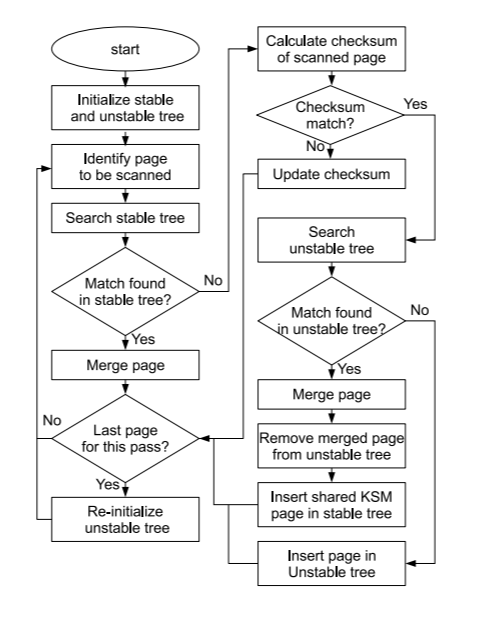
\includegraphics[width=\linewidth]{_summaries/deduplication/_images/ksm-algo.png}
  \caption{KSM Algorithm}
  \label{fig:ksm1}
\end{figure}

\subsubsubsection{API}
KSM is a Linux kernel thread that run independently on demand when virtual areas is registered as mergeable.

\begin{minted}{cpp}
#include <sys/mman.h>

int madvise(void *addr, size_t length, int advice);
\end{minted}

\textbf{int advice:}
\begin{itemize}
\item \textbf{MADV\_MERGEABLE} (since Linux 2.6.32) \\
  Enable Kernel Samepage Merging (KSM) for the pages in the
  range specified by addr and length.  The kernel regularly
  scans those areas of user memory that have been marked as
  mergeable, looking for pages with identical content.  These
  are replaced by a single write-protected page (which is
  automatically copied if a process later wants to update the
  content of the page).  KSM merges only private anonymous pages
  (see mmap(2)).
  
  The KSM feature is intended for applications that generate
  many instances of the same data (e.g., virtualization systems
  such as KVM).  It can consume a lot of processing power; use
  with care.  See the Linux kernel source file
  Documentation/admin-guide/mm/ksm.rst for more details.

  The \textbf{MADV\_MERGEABLE} and \textbf{MADV\_UNMERGEABLE} operations are
  available only if the kernel was configured with \textbf{CONFIG\_KSM}.

\item \textbf{MADV\_UNMERGEABLE} (since Linux 2.6.32) \\
  Undo the effect of an earlier \textbf{MADV\_MERGEABLE} operation on the
  specified address range; KSM unmerges whatever pages it had
  merged in the address range specified by addr and length.
\end{itemize}

\vspace{5mm}

\textbf{Caveats:}
\begin{itemize}
\item KSM is possible to scan all anonymous page but it should be wasteful where we cannot find equal anonymous pages.

\item To keep track of the pages, KSM uses \textbf{Slab Allocation}. \\ The number of slab allocation is linearly increasing with the size of registered virtual areas.
\end{itemize}

\vspace{5mm}

\textbf{The KSM behavior can be controlled through sysfs at /sys/kernel/mm/ksm/:}
\begin{itemize}
\item \textbf{run}
  \begin{itemize}
  \item 1 for running
  \item 0 for stop
  \item 2 for stop ksmd and unmerge all pages currently merged, but leave mergeable areas registered for next run
  \end{itemize}
\item \textbf{pages\_to\_scan} -> how many pages to scan before ksmd go to sleep, e.g. 100
\item \textbf{sleep\_millisecs} -> how many milliseconds ksmd should sleep before next scan, e.g. 20
\item \textbf{merge\_across\_nodes} -> specifies if pages from different NUMA nodes can be merged
  \begin{itemize}
  \item 0 -> ksm merges only pages which physically reside in the memory area of same NUMA node. That brings lower latency to access of shared pages. Systems with more nodes, at significant NUMA distances, are likely to benefit from the lower latency
  \item 1 (default) -> Smaller systems, which need to minimize memory usage, are likely to benefit from the greater sharing
  \end{itemize}
\item \textbf{use\_zero\_pages} -> specifies whether empty pages (i.e. allocated pages that only contain zeroes) should be treated specially
  \begin{itemize}
  \item 0, normal behavior
  \item 1, empty pages are merged with the kernel zero page(s) instead of with each other as it would happen normally. This can improve the performance on architectures with coloured zero pages, depending on the workload. Care should be taken when enabling this setting, as it can potentially degrade the performance of KSM for some workloads, for example if the checksums of pages candidate for merging match the checksum of an empty page
  \end{itemize}
\item \textbf{max\_page\_sharing} -> Maximum sharing allowed for each KSM page, to avoid high latency for virtual memory operations that involve traversal of virtual mappings that share the KSM page
\item \textbf{stable\_node\_chains\_prune\_millisecs} -> specifies how frequently KSM checks the metadata of the pages that hit the deduplication limit for stale information
\end{itemize}

\vspace{5mm}

\textbf{The KSM effectiveness can be seen through sysfs at /sys/kernel/mm/ksm/ with this parameter:}
\begin{itemize}
\item \textbf{pages\_shared} -> how many shared pages are being used
\item \textbf{pages\_sharing} -> how many more sites are sharing them i.e. how much saved
\item \textbf{pages\_unshared} -> how many pages unique but repeatedly checked for merging
\item \textbf{pages\_volatile} -> how many pages changing too fast to be placed in a tree
\item \textbf{full\_scans} -> how many times all mergeable areas have been scanned
\item \textbf{stable\_node\_chains} -> the number of KSM pages that hit the \textbf{max\_page\_sharing} limit
\item \textbf{stable\_node\_dups} -> number of duplicated KSM pages
\end{itemize}

\vspace{5mm}

\subsubsubsection{Sum up}
\begin{enumerate}
\item KSM is to increase memory density
\item KSM is generating shared pages by merging equal pages, and in turn it is making free memory available allowing to run more virtual machines or applications on the same system, than otherwise would be possible without KSM
\item A high ratio of \textbf{pages\_sharing} to \textbf{pages\_shared} indicates good sharing, but a high ratio of \textbf{pages\_unshared} to \textbf{pages\_sharing} indicates wasted effort. \textbf{pages\_volatile} embraces several different kinds of activity, but a high proportion there would also indicate poor use of madvise \textbf{MADV\_MERGEABLE}.
\end{enumerate}